\documentclass{beamer}


	\usetheme{Madrid}

\usepackage[utf8]{inputenc}

\usepackage[slovak]{babel}



\title{Uhlové korelácie s podivnými časticami}
\author{ \bf  Lucia Anna Husová}
\institute[]{
\includegraphics[scale=0.3]{logo.png}{\vspace{.3cm}}\\ \bf Katedra jadrovej a subjadrovej fyziky \\ Prírodovedecká fakulta\\ {\bf Univerzita Pavla Jozefa Šafárika\vspace{.3cm}} \\ {\bf Školiteľ: RNDr. Marek Bombara, PhD\vspace{.3cm}}\\ {\bf ALICE Workshop - Danišovce}}
\date{06.06.2017 }

\begin{document}
	\maketitle

\begin{frame}
	\frametitle{Obsah}
		\tableofcontents
\end{frame}	


\section{Úvod do problematiky}
	\begin{frame}
	\frametitle{Jety}
		\begin{itemize}
			\item Práca vykonaná na oddelenie kvarkov resp. gluónov sa mení na energiu poľa, z ktorej vzniká spŕška hadrónov v jednom smere - tzv. jet
		\end{itemize}
			\begin{columns}
				\begin{column}{0.6\textwidth}
				\centering{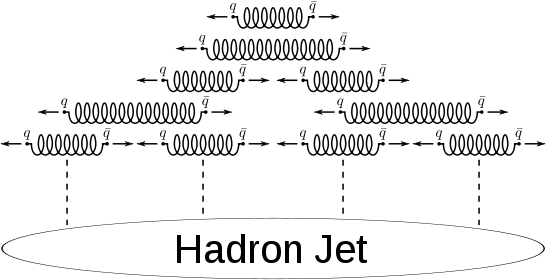
\includegraphics[scale=0.3]{../Obrazky_praca/jet.png}}
				\end{column}
				\begin{column}{0.4\textwidth}
					\centering{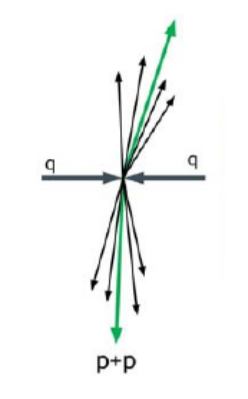
\includegraphics[scale=0.4]{../Obrazky_praca/jetschema.png}}
				\end{column}
			\end{columns}
 		\end{frame}	

	\begin{frame}
		\frametitle{Metóda dvojčasticových korelácií}
		\begin{itemize}
			\item Nepriama metóda na skúmanie jetov
			\item Trigrovacia častica - vysoká priečna hybnosť, asociované častice - nižšia priečna hybnosť
			\item [] $ \Delta \phi = \phi_{trig} - \phi_{asoc} $
			\item [] $\Delta \eta = \eta_{trig} - \eta_{asoc}$
			\item [] \centering 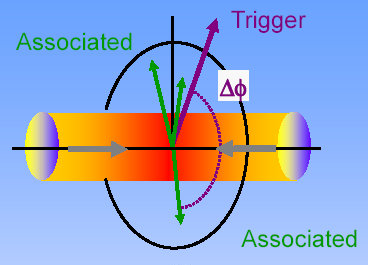
\includegraphics[scale=0.4]{../Obrazky_praca/dihadron.png}
		\end{itemize}
	\end{frame}
	
	\begin{frame}
		\frametitle{Počítanie výťažkov}
		\begin{columns}
			\begin{column}{0.5\textwidth}
				\begin{itemize}
					\item korekcie:
					\begin{itemize}
						\item konečná akceptancia detektora
						\item účinnosť rekonštrukcie dráh asociovaných častíc
						\item normovanie na počet trigrovacích častíc
						\item odpočítanie pozadia
					\end{itemize}
				\end{itemize}
			\end{column}
		\begin{column}{0.5\textwidth}
			\centering 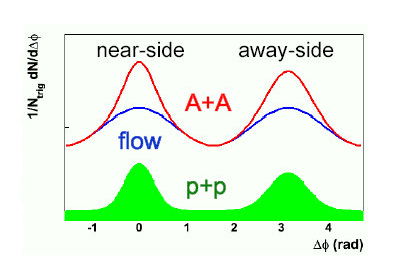
\includegraphics[scale=0.5]{../Obrazky_praca/DetaPhiSchema.png}
		\end{column}
		\end{columns}
		\begin{itemize}
			\item {\bf výťažok} - priemerný počet asociovaných častíc na jednú trigrovaciu časticu pri danej priečnej hybnosti
			\begin{equation}
			Y_J^{\Delta\phi}=\int_{\Delta \phi_1}^{\Delta \phi_2} \frac{d^2N}{d\Delta \phi } d\Delta\phi 
			\label{yield}
			\end{equation} 
		\end{itemize}
	\end{frame}

\section{Ciele práce}
	
	\begin{frame}
		\frametitle{Ciele práce}
		\begin{itemize}
			\item Vypracovanie všeobecného kódu použiteľného na analýzu identifikovaných a neidentifikovaných dvojhadrónových korelácií na všetky typy zrážok pri rôznych energiách
			\item Testovanie kódu na dátach z protónovo-protónových zrážok pri 13 TeV (vysoká štatistika, nízke pozadie)
			\begin{itemize}
				\item Testovanie metódy na h-h koreláciach
				\item Analýza korelácií s identikovanými trigrovacími časticami (podivné častice)
				\item Porovnanie výsledkov s MC generovanými dátami 
			\end{itemize}
		\end{itemize}
	\end{frame}

\section{Metóda merania}

	\subsection{Spracované dáta a selekčné kritéria}
	\begin{frame}
		\frametitle{Spracované dáta a selekčné kritéria}
		\begin{itemize}
			\item Protónovo-protónové zrážky pri energii $\sqrt{s}=13$ TeV z roku 2015
			\item $1.17\times10^7$ prefiltrovaných zrážok 
			\item Výpočet prebehol na gride AliEn
			\item Optimalizované selekčné kritéria pre nabité hadróny a V0 častice
			\item 4 GeV/c $<p_T^{trig}$
			\item 2 GeV/c$<p_T^{asoc}<p_T^{trig}$
			\item Trigrovacie častice
			\begin{itemize}
				\item Nabité neidentifikované primárne hadróny
				\item Podivné hadróny ($K^0_S$,$\Lambda$) - dobrá identifikácia aj pre vysoké $p_T$
			\end{itemize}
		\end{itemize}
	\end{frame}

	\begin{frame}
	\frametitle{Výberové kritéria pre V0 častice}
	\begin{table}[hbtp!]
		\begin{center}
			\begin{tabular}{|c|c|}
				\hline
				\multicolumn{2}{|c|}{Selekčné kritéria pre V0}  \\ \hline
				$K^0_S$ & $\Lambda$ + $\bar{\Lambda}$ \\ \hline
				$cos\theta_{PA} >0.97$ & $cos\theta_{PA} >0.995$  \\ \hline
				$|y|<0.75$ & $|y|<0.75$   \\ \hline
				DCA Neg$>$0.06 cm & DCA Neg$>$0.06 cm \\ \hline
				DCA Pos$>$0.06 cm & DCA Pos$>$0.06 cm \\ \hline
				DCA V0 daughters$<$ 1 cm & DCA V0 daughters $<$1 cm \\ \hline
				lifetime$<$20 cm & lifetime$<$30 cm \\ \hline
				V0 2D Decay Radius $>$ 0.5 & V0 2D Decay Radius $>$ 0.5\\ 
				\hline
			\end{tabular}
			\caption{Tabuľka selekčných kritérii pre V0 častice}
			\label{tabulka}
		\end{center}
	\end{table}

	\end{frame}

	\begin{frame}
		\frametitle{Výberové kritéria pre V0 častice}
		\centering 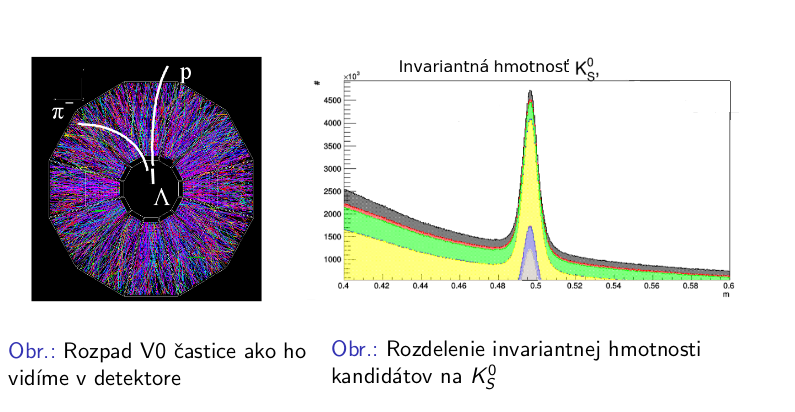
\includegraphics[scale=0.6]{../Obrazky_praca/SelekcneV0.png}
			
	\end{frame}

	\begin{frame}
		\frametitle{Dvojčasticové korelácie}
		\centering 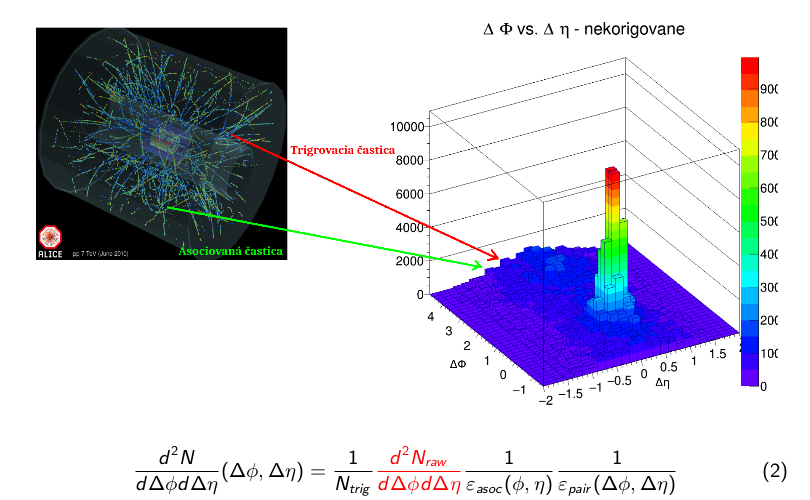
\includegraphics[scale=0.55]{../Obrazky_praca/siblings.png}
	\end{frame}

\subsection{Korekcie}

	\begin{frame}
		\frametitle{Korekcia na konečnú akceptanciu detektora}
		\centering 
		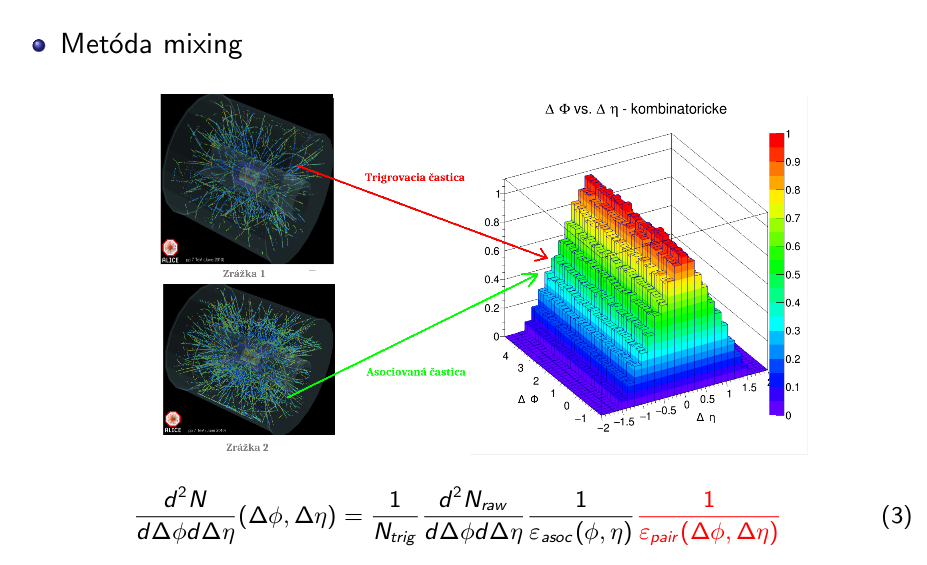
\includegraphics[scale=0.5]{../Obrazky_praca/mixing.png}
	\end{frame}

	\begin{frame}
		\frametitle{Korekcia na účinnosť rekonštrukcie asociovaných častíc v detektore}
		\begin{center}
			\begin{itemize}
				\item[] \centering 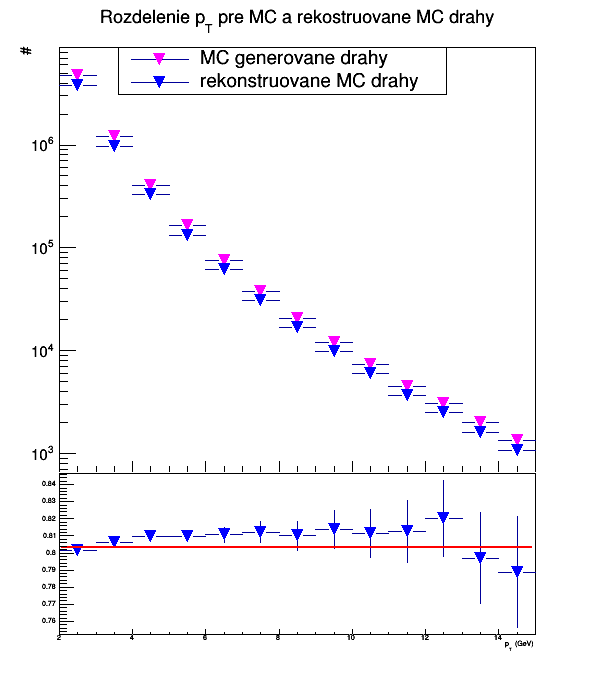
\includegraphics[scale=0.25]{../Obrazky_praca/MC_closure.png}
				\item[] $\frac{d^2N}{d\Delta\phi d\Delta\eta}(\Delta\phi,\Delta \eta) = \frac{1}{N_{trig}} \frac{d^2N_{raw}}{d\Delta\phi d\Delta\eta} \textcolor{red}{\frac{1}{\epsilon_{asoc}(\phi,\eta)}}\frac{1}{\epsilon(\Delta\phi,\Delta\eta)}$
			\end{itemize}
		\end{center}
	
			
		
	\end{frame}

\subsection{Výťažky}

	\begin{frame}
		\frametitle{Príklad rozdelenia $\Delta \phi$}
		\centering 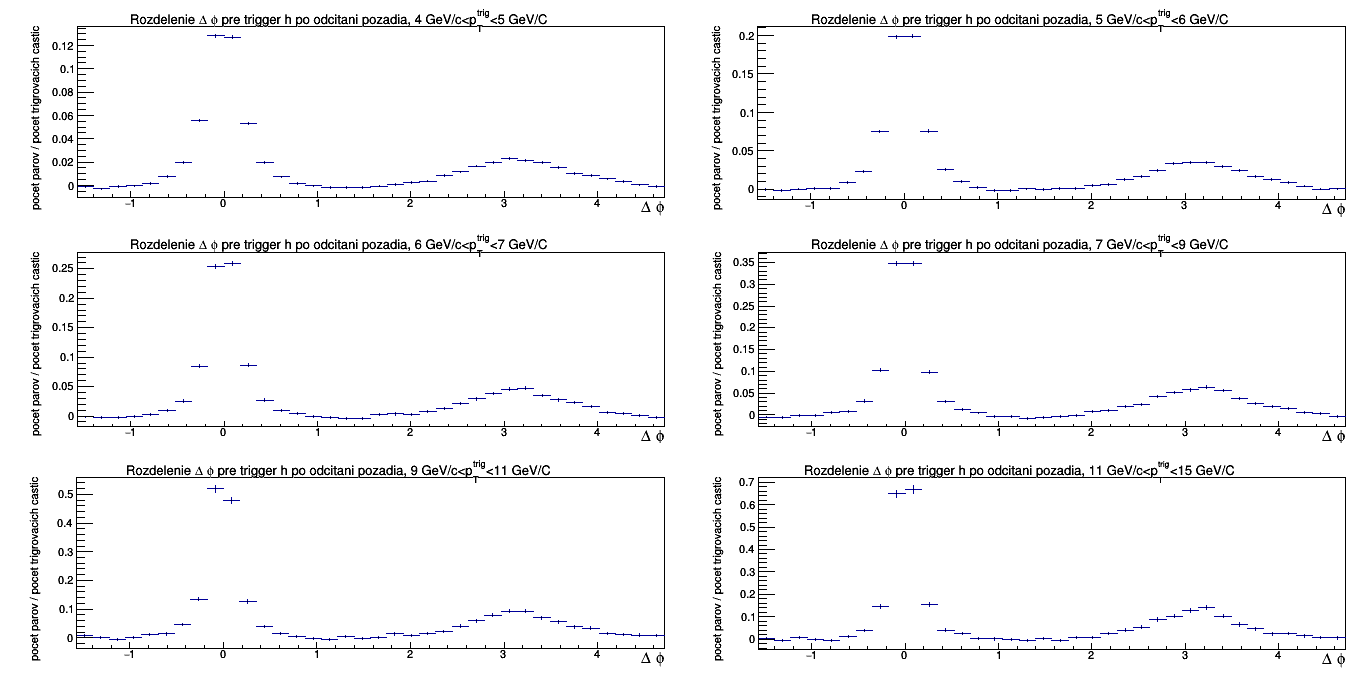
\includegraphics[scale=0.25]{../Obrazky_praca/DeltaPhiHH.png}
		
		$Y_J^{\Delta\phi}=\int_{\Delta \phi_1}^{\Delta \phi_2} \frac{dN}{d\Delta \phi } d\Delta\phi $
	\end{frame}

\section{Výsledky}

	\begin{frame}
		\frametitle{Výťažky pre priľahlý pík}
		\centering 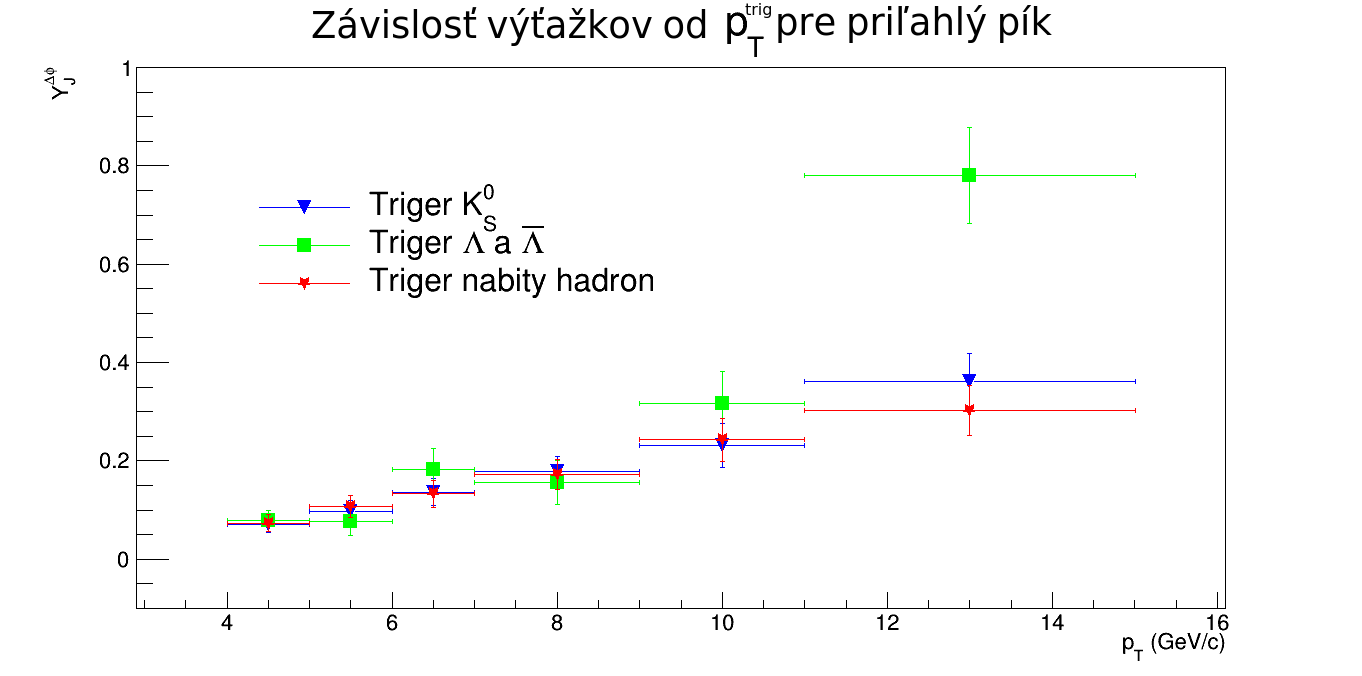
\includegraphics[scale=0.35]{../Obrazky_praca/vytazok_near.png}

	\end{frame}

	\begin{frame}
		\frametitle{Výťažky pre pritiľahlý pík}
		\centering 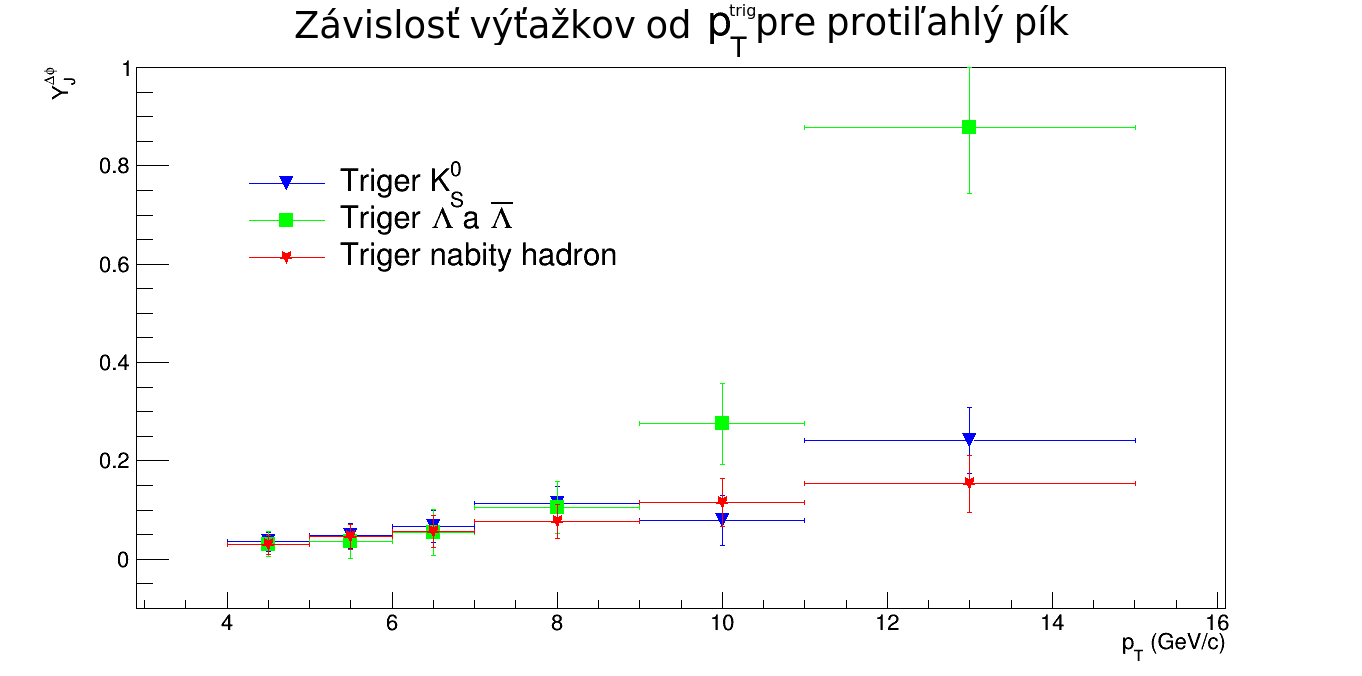
\includegraphics[scale=0.35]{../Obrazky_praca/vytazok_away.png}
	
	\end{frame}

	\begin{frame}
	\frametitle{MC porovnanie pre h-h korelácie}
		\centering 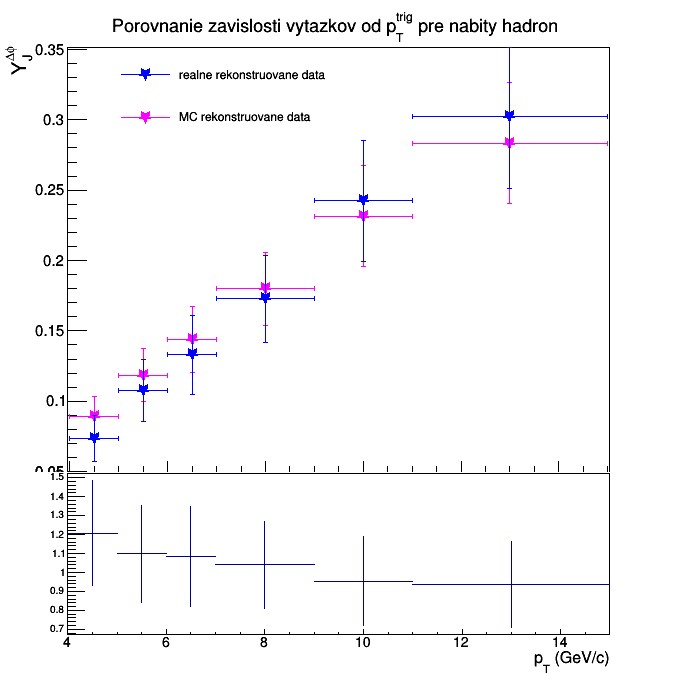
\includegraphics[scale=0.3]{../Obrazky_praca/Vytazok_porovnanieMCh.png}
	
	\end{frame}

\begin{frame}
\frametitle{MC porovnanie pre $K^0_S$-h korelácie}
\centering 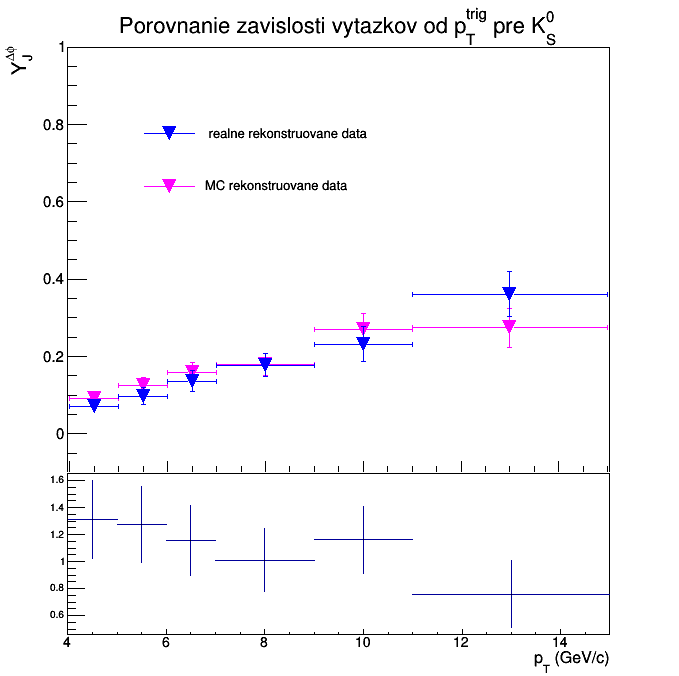
\includegraphics[scale=0.3]{../Obrazky_praca/Vytazok_porovnanieMC.png}

\end{frame}

\begin{frame}
\frametitle{MC porovnanie pre $(\Lambda+\bar{\Lambda})$-h korelácie}
\centering 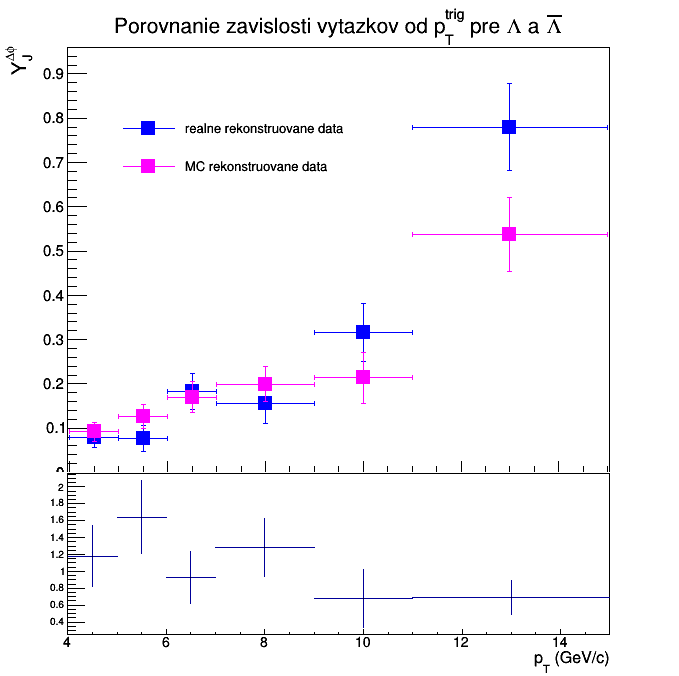
\includegraphics[scale=0.3]{../Obrazky_praca/Vytazok_porovnanieMCl.png}

\end{frame}

\section{Zhrnutie}

\begin{frame}
	\frametitle{Zhrnutie}
	\begin{itemize}
		\item Aplikácia všeobecného kódu na zrážky protón-protón
		\item Výpočet výťažkov pre korelácie s určenou a neurčenou trigrovacou časticou
		\item Rast výťažkov s rastúcou priečnou hybnosťou trigrovacej častice
		\item Nemožnosť určenia presného poradia veľkosti výťažkov pre jednotlivé trigrovacie častice
		\item MC dobre popisuje závislosť výťažkov od priečnej hybnosti trigrovacej častice
		\item V budúcnosti - aplikácia metódy na jadrovo-jadrové zrážky
	\end{itemize}
\end{frame}

	\begin{frame}
	 \centering	\LARGE Ďakujem za pozornosť!	
	\end{frame}

\end{document}
